% =============================================================================
\section{El 2 de octubre: ultrasónico y buzzer}
% =============================================================================

\begin{frame}{El robot terminado}
  \centering
  \includegraphics[height=0.37\textheight]{robot_terminado_lado.jpg}\hspace{1.5mm}%
  \includegraphics[height=0.37\textheight]{robot_terminado_arriba.jpg}\hspace{1.5mm}%
  \includegraphics[height=0.37\textheight]{robot_terminado_frente.jpg}

  \vspace{0.3em}
  \relax{\footnotesize
  \begin{columns}[T,onlytextwidth]
    \begin{column}{0.485\textwidth}
      \begin{block}{Qué se ve}
        \begin{itemize}
          \item Al frente, sobre una protoboard amarilla, el \textbf{ultrasónico}
                (los dos ``ojos''), y arriba la \textbf{webcam}.
          \item En la protoboard blanca, el \textbf{ESP32}, el divisor del
                sensor y el \textbf{buzzer} (el cilindro negro).
          \item Al lado, la \textbf{Raspberry Pi 5}; atrás, el \textbf{L298N}
                (rojo) y los dos motores.
          \item Debajo, la caja negra con las baterías.
        \end{itemize}
      \end{block}
    \end{column}
    \begin{column}{0.485\textwidth}
      \begin{block}{Qué cambió respecto del 1 de octubre}
        El día anterior se había decidido dejar el ultrasónico y el buzzer para
        una segunda versión, por tiempo. El 2 de octubre se \textbf{revirtió}:
        la idea era agregar el ultrasónico ``en media hora'', para que el robot
        no chocara contra las paredes al huir.
      \end{block}
      \begin{alertblock}{Lo que llevó}
        Algo más de \textbf{dos horas}, y entró también el buzzer. Las fotos
        están en \cod{Fotos del bot/}.
      \end{alertblock}
    \end{column}
  \end{columns}}
\end{frame}

\begin{frame}{Cómo quedó cableado}
  \begin{columns}[T,onlytextwidth]
    \begin{column}{0.50\textwidth}
      \relax{\footnotesize
      \begin{tabular}{L{2.1cm}L{0.9cm}L{3.2cm}}
        \toprule
        \textbf{Señal} & \textbf{GPIO} & \textbf{Nota} \\
        \midrule
        PING))) \textbf{SIG} & \textbf{12} & Con divisor. Disparo y eco por el mismo pin \\[1pt]
        PING))) \textbf{5V} & VIN & 5 V del USB \\[1pt]
        PING))) \textbf{GND} & GND & Común con el ESP32 \\[1pt]
        Buzzer \textbf{+} & \textbf{14} & Activo, de dos patas, directo \\[1pt]
        Buzzer \textbf{--} & GND & \\
        \bottomrule
      \end{tabular}}

      \vspace{0.2em}
      \centering
      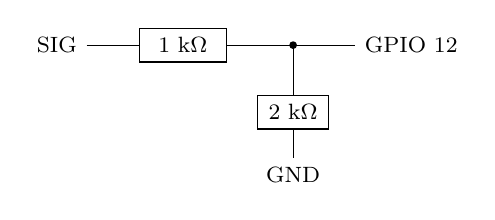
\begin{tikzpicture}[font=\footnotesize]
        \node (sig) at (0,0) {SIG};
        \node[draw, minimum width=1.1cm, minimum height=0.36cm] (r1) at (1.6,0) {1 k$\Omega$};
        \coordinate (n) at (3.0,0);
        \node (gpio) at (4.5,0) {GPIO 12};
        \node[draw, minimum width=0.9cm, minimum height=0.36cm] (r2) at (3.0,-0.85) {2 k$\Omega$};
        \node (gnd) at (3.0,-1.65) {GND};
        \draw (sig) -- (r1) -- (n) -- (gpio);
        \fill (n) circle (1.4pt);
        \draw (n) -- (r2) -- (gnd);
      \end{tikzpicture}
    \end{column}
    \begin{column}{0.47\textwidth}
      \relax{\footnotesize
      \begin{block}{Por qué el divisor}
        El sensor contesta a \textbf{5 V} y el ESP32 no los tolera. Hacia el
        ESP32 baja a 3,3 V; hacia el sensor, el disparo llega a 3,3 V por la
        de 1 k$\Omega$, que alcanza (la entrada es TTL).
        \ojo{Cruzadas}, el eco llega a 1,7 V y el sensor parece mudo.
      \end{block}
      \begin{block}{Por qué esos pines}
        El plan era el 19 para el sensor y el 4 para el buzzer. En la
        protoboard sólo queda accesible \textbf{una fila} del ESP32, y de esa
        fila los únicos libres que pueden ser salida son el 12 y el 14.
      \end{block}
      \begin{alertblock}{Dos trampas de pines}
        \begin{itemize}
          \item El \textbf{35} es de sólo entrada: el buzzer se conectó ahí
                primero, y ahí no suena.
          \item El \textbf{12} es pin de arranque: en alto al salir del reset,
                el ESP32 no arranca. La de 2 k$\Omega$ lo tiene en bajo.
        \end{itemize}
      \end{alertblock}}
    \end{column}
  \end{columns}
\end{frame}

\begin{frame}{El firmware: un sensor de un solo pin}
  \relax{\footnotesize
  \begin{columns}[T,onlytextwidth]
    \begin{column}{0.485\textwidth}
      \begin{block}{Qué había y qué hizo falta}
        El firmware estaba escrito para un HC-SR04, con un pin para disparar y
        otro para el eco. El \textbf{Parallax PING)))} usa uno solo: el ESP32
        manda el pulso de disparo y enseguida escucha por el mismo cable.
      \end{block}
      \begin{block}{Cómo se hace}
        \begin{enumerate}
          \item El pin pasa a \textbf{salida} y da un pulso de 5 $\mu$s.
          \item Pasa a \textbf{entrada}. El sensor espera 750 $\mu$s antes de
                contestar: sobra tiempo.
          \item Una interrupción mide el ancho del pulso de eco: 58 $\mu$s por
                centímetro.
        \end{enumerate}
        La interrupción sólo mira dentro de la \textbf{ventana de escucha}:
        así el propio disparo nunca se toma por un eco.
      \end{block}
    \end{column}
    \begin{column}{0.485\textwidth}
      \begin{block}{Lo que hay que saber de las lecturas}
        \begin{itemize}
          \item \textbf{$\sim$370 cm es ``libre''}: sin nada adelante el sensor
                devuelve su pulso más largo. No es una distancia.
          \item \textbf{$-1$ es ``no contestó''}: sensor desconectado. El Pi lo
                lee como ``no sé'', no como distancia cero.
          \item Mide de 2 cm a 3 m, cada 60 ms.
        \end{itemize}
      \end{block}
      \begin{block}{Lo que quedó en el firmware}
        \begin{itemize}
          \item \cod{PIN_SONAR} 12, \cod{PIN_BUZZER} 14, \cod{BUZZER_PASSIVE} 0.
          \item Tecla \cod{e}: contadores del sensor (disparos, flancos, ecos).
          \item Tecla \cod{u}: un disparo y la línea mirada con el ADC.
          \item Tecla \cod{U}: línea en alto fijo, para medirla con el tester.
        \end{itemize}
      \end{block}
    \end{column}
  \end{columns}}
\end{frame}

\begin{frame}{El primer sensor estaba muerto: cómo se descartó todo lo demás}
  \relax{\footnotesize
  \begin{tabular}{L{6.2cm}L{7.4cm}}
    \toprule
    \textbf{Prueba} & \textbf{Qué descartó} \\
    \midrule
    Contadores de disparos, entradas a la interrupción y ecos &
      La interrupción: ve exactamente 2 flancos por disparo, los del propio
      pulso \\[1pt]
    Leer el pin con el pull-up interno puesto &
      Que el divisor no estuviera en ese pin: lee 0, hay camino a GND \\[1pt]
    La línea mirada con el ADC durante 25 ms después del disparo &
      Un eco a media altura por las resistencias cruzadas: 0,00 V \\[1pt]
    Disparos de 5, 20, 100 y 1000 $\mu$s &
      El ancho del disparo \\[1pt]
    Línea en alto fijo, medida con el tester sobre los pines del sensor &
      El cableado: 3,3 V en SIG y 5 V en la alimentación \\
    \bottomrule
  \end{tabular}}

  \vspace{0.5em}
  \relax{\footnotesize
  \begin{columns}[T,onlytextwidth]
    \begin{column}{0.485\textwidth}
      \begin{block}{El resultado}
        Con todo eso bien, el sensor seguía mudo. Cambiado por otro igual:
        \textbf{30 cm clavados, 120 de 120 lecturas}, con una caja a 30 cm.
        Costó unos 20 minutos.
      \end{block}
    \end{column}
    \begin{column}{0.485\textwidth}
      \begin{block}{Por qué se hizo así}
        Con todas las lecturas en $-1$ no se sabe si falla el firmware, el
        cableado o el sensor. Cada prueba se agregó al firmware para descartar
        una causa \textbf{sin pedirle al usuario que revisara a ciegas}. El
        procedimiento quedó en el \cod{RUNBOOK.md}, Paso 25.
      \end{block}
    \end{column}
  \end{columns}}
\end{frame}

\begin{frame}{Cómo usa el Pi la distancia}
  \relax{\footnotesize
  \begin{columns}[T,onlytextwidth]
    \begin{column}{0.485\textwidth}
      \begin{block}{Dos umbrales}
        \begin{itemize}
          \item \cod{DIST_PARADA_CM} = \textbf{20}: el de \emph{llegada}. En
                \cod{APROXIMAR}, algo a menos de 20 cm cuenta como llegada si es
                el oso; si no, se desvía.
          \item \cod{DIST_OBSTACULO_CM} = \textbf{30}: el de \emph{esquivar}. En
                la fase 3 de \cod{HUIR} y en el pulso de avance de
                \cod{BUSCAR}: no avanza, \textbf{gira en el lugar}.
        \end{itemize}
        Al oso hay que poder acercarse; a una pared, no.
      \end{block}
      \begin{block}{Retención: 0,3 s}
        Un obstáculo se da por cierto hasta 0,3 s después de la última lectura
        que lo vio (\cod{SONAR_RETENCION_S}). Girando frente a una pared el eco
        se pierde de a ratos y aparece un ``libre'' falso.
      \end{block}
    \end{column}
    \begin{column}{0.485\textwidth}
      \begin{block}{¿El eco es el oso?}
        Si el oso está a la vista con $|error_x| < 0{,}7$ y ya ocupa el 60 \%
        del área objetivo, lo que hay adelante es él. El 0,7 sale del cono del
        sensor ($\pm$20\grad) contra el semicampo de la cámara (26\grad).
      \end{block}
      \begin{alertblock}{Lo que el sensor no arregla}
        \begin{itemize}
          \item \textbf{Sólo mira adelante.} El retroceso y el giro de la huida
                siguen a ciegas: las lecturas más bajas del día (7 y 13 cm)
                fueron al terminar el giro, no avanzando.
          \item \textbf{Una pared muy de costado no la ve} hasta estar encima:
                el eco rebota para otro lado.
          \item \textbf{Sin lectura, el robot anda igual pero a ciegas.}
                \cod{main.py} lo avisa al arrancar.
        \end{itemize}
      \end{alertblock}
    \end{column}
  \end{columns}}
\end{frame}

\begin{frame}{El día, prueba por prueba}
  \relax{\footnotesize
  \begin{tabular}{L{1.1cm}L{3.6cm}L{8.9cm}}
    \toprule
    \textbf{Dónde} & \textbf{Prueba} & \textbf{Qué pasó} \\
    \midrule
    banco & Primer sensor & Todas las lecturas en $-1$. Cinco pruebas después:
      el sensor está muerto. \\[1pt]
    banco & Segundo sensor & 30 cm con una caja a 30 cm, 120 de 120. \\[1pt]
    piso & Quieto, pared a 1,5 m & 153 cm, estable. Sin ecos del piso. \\[1pt]
    piso & Avance hasta leer 20 cm & A velocidad 40: manda frenar leyendo 19 y
      queda a \textbf{16 cm}. \\[1pt]
    10:34 & Huida, pared a 1 m & El avance terminó solo a 27 cm: el sensor no
      llegó a actuar. \\[1pt]
    10:36 & Huida, pared a 80 cm & \textbf{Esquiva}: corta a 18 cm y gira.
      Después lee 16, \textbf{150}, 11 y avanza un ciclo. \\[1pt]
    10:41 & Demo del oso & Se acerca sin desvíos falsos (119 a 28 cm) y frena
      por tamaño. \\[1pt]
    10:54 & (cable del sensor suelto) & \ojo{553 filas sin lectura}: 52 s a
      ciegas, cortada a mano. \\[1pt]
    10:59 & Con dos umbrales y buzzer & Corta el avance a \textbf{29 cm}; no
      baja de 27. Suena en los tres momentos. \\[1pt]
    11:07 & Grabada (la del video) & Huye a los 2 s, esquiva a 29 cm, encuentra
      el oso a los 8 s. \\
    \bottomrule
  \end{tabular}}

  \vspace{0.3em}
  {\footnotesize Seis corridas con el programa completo, \textbf{3675 frames y
  ninguno con franjas}. Al mediodía: 69 verificaciones (eran 60); a la tarde, 79.}
\end{frame}

\begin{frame}{Tres ajustes, cada uno por una corrida}
  \relax{\footnotesize
  \begin{columns}[T,onlytextwidth]
    \begin{column}{0.32\textwidth}
      \begin{block}{1. El oso descentrado}
        Al llegar, oso grande pero corrido a la derecha ($+0{,}53$) y el sensor
        en 22 cm. Con 20 lo habría tomado por un obstáculo ajeno y habría
        girado a tope para el otro lado.

        \vspace{0.3em}
        \cod{SONAR_CENTRADO}: \textbf{0,35 \hacia{} 0,7}. La regla pedía un oso
        más centrado de lo que el sensor distingue.
      \end{block}
    \end{column}
    \begin{column}{0.32\textwidth}
      \begin{block}{2. La lectura suelta}
        Girando frente a la pared: 16 cm, \textbf{150}, 11. Con el 150 avanzó
        un ciclo contra la pared.

        \vspace{0.3em}
        \cod{SONAR_RETENCION_S} = \textbf{0,3}. En la corrida siguiente apareció
        un 172 entre lecturas de 12--16 y el robot no avanzó.
      \end{block}
    \end{column}
    \begin{column}{0.32\textwidth}
      \begin{block}{3. Poco margen}
        Con un solo umbral de 20 cm, en las huidas la lectura bajó a 16, 11 y
        12 cm: el robot no frena, pivotea, y el frente barre un arco.

        \vspace{0.3em}
        \cod{DIST_OBSTACULO_CM} = \textbf{30}, aparte del de llegada. Corta a
        29 y no baja de 27.
      \end{block}
    \end{column}
  \end{columns}}

  \vspace{0.6em}
  \begin{alertblock}{Los tres valen por una sola corrida}
    \footnotesize Son ajustes a ojo, hechos sobre lo que mostró el registro.
    Ninguno tiene una serie de mediciones detrás.
  \end{alertblock}
\end{frame}

\begin{frame}{Lo que falló ese día, fuera del sensor}
  \relax{\footnotesize
  \begin{columns}[T,onlytextwidth]
    \begin{column}{0.485\textwidth}
      \begin{block}{El estreno de los comandos de la noche anterior}
        \begin{itemize}
          \item \cod{demo.sh correr}, con la webcam desenchufada, mostraba el
                análisis de la corrida \textbf{del día anterior} como si fuera
                el de ésta. Ahora dice que no se hizo.
          \item \cod{traer_corrida.ps1} no copiaba nada: la ruta tiene
                espacios y terminaba en barra invertida. Y elegía el
                \cod{.avi} en vez del \cod{.mp4}.
          \item \cod{demo.sh firmware}, en su primer uso tras encender:
                ``comando desconocido''.
        \end{itemize}
        Los tres corregidos. El \cod{hotspot} se cargó y se probó al cierre:
        el Pi arranca en él. Sin estrenar: \cod{fondo}.
      \end{block}
      \begin{block}{Una corrida a ciegas}
        Se soltó un cable del sensor y nadie lo supo hasta ver el robot. Y al
        cancelar desde la PC, \textbf{el programa siguió andando en el Pi}.
        Quedaron el aviso de \cod{main.py} al arrancar y \cod{demo.sh sonar}.
      \end{block}
    \end{column}
    \begin{column}{0.485\textwidth}
      \begin{alertblock}{Bajo voltaje con las baterías cargándose}
        Con las baterías enchufadas a sus cargadores, el Pi marcó bajo voltaje
        en reposo: 4,72--4,80 V. Desconectadas: 5,10 V y \cod{0x0}. Visto dos
        veces el mismo día.
      \end{alertblock}
      \begin{alertblock}{La webcam se había soltado}
        Al bajar el robot al piso, el Pi dejó de verla. Reinsertada: cero
        franjas en 3675 frames.
      \end{alertblock}
      \begin{block}{Qué dice eso de la imagen rota del 1 de octubre}
        Que la causa puede haber sido el enchufe o la alimentación. Pero ese
        día cambiaron \textbf{las dos cosas a la vez}, así que no se sabe cuál.
        Sigue sin aislar.
      \end{block}
    \end{column}
  \end{columns}}
\end{frame}

\begin{frame}{Lo que cambió ese día}
  \relax{\footnotesize
  \begin{tabular}{L{3.6cm}L{2.2cm}L{2.5cm}L{5.3cm}}
    \toprule
    \textbf{Qué} & \textbf{Antes} & \textbf{Después} & \textbf{Por qué} \\
    \midrule
    Ultrasónico & sin cablear & PING))) en el GPIO 12 & Que no avance contra una pared \\
    Buzzer & sin cablear & activo, en el GPIO 14 & Avisar la huida y la llegada \\
    Firmware, sensor & HC-SR04, 2 pines & un solo pin & El sensor que había \\
    \cod{BUZZER_PASSIVE} & 1 & 0 & El buzzer es activo \\
    Pulso de avance de \cod{BUSCAR} & avanza siempre & gira si hay algo & Era el único avance sin mirar \\
    \cod{DIST_OBSTACULO_CM} & --- & 30 & Con 20, la lectura bajaba a 11 cm \\
    \cod{SONAR_RETENCION_S} & --- & 0,3 & Una lectura libre suelta hacía avanzar \\
    \cod{SONAR_CENTRADO} & 0,35 & 0,7 & El robot llega descentrado \\
    \cod{main.py} & --- & avisa si no hay lectura & Una corrida entera salió a ciegas \\
    \cod{demo.sh} & 12 comandos & 13: \cod{sonar} & Ver el sensor sin mover el robot \\
    Scripts de \cod{piso/} & --- & \cod{sonar.py}, \cod{freno_sonar.py} & Medir quieto, y dónde queda al frenar \\
    Barrido después de huir & siempre a la derecha & sorteado, o lejos de la mochila & Huía en ciclo: seis veces en un minuto \\
    Verificaciones & 60 & 79 & Los casos nuevos del sensor y del barrido \\
    \bottomrule
  \end{tabular}}

  \vspace{0.4em}
  {\footnotesize El detalle está en \cod{PLAN.md} §13, Día 15, y en
  \cod{HARDWARE.md} §9.}
\end{frame}
